\documentclass[aspectratio=169,10pt]{beamer}

\usefonttheme{professionalfonts}
\setbeamertemplate{navigation symbols}{}

\usepackage{graphicx}
\usepackage{booktabs}
\usepackage{hyperref}
\usepackage{amsmath}
\usepackage{ragged2e}
\usepackage{xcolor}

\definecolor{SCUGreen}{RGB}{8,79,52}
\definecolor{SCULight}{RGB}{223,233,227}
\definecolor{SCUDot}{RGB}{35,137,79}
\definecolor{SCUText}{RGB}{41,63,70}

\setbeamercolor{background canvas}{bg=white}
\setbeamercolor{normal text}{fg=SCUText,bg=white}
\setbeamercolor{title}{fg=SCUGreen}
\setbeamercolor{subtitle}{fg=SCUGreen}
\setbeamercolor{frametitle}{fg=SCUGreen,bg=SCULight}
\setbeamercolor{itemize item}{fg=SCUDot}
\setbeamercolor{itemize subitem}{fg=SCUDot}
\setbeamercolor{enumerate item}{fg=SCUDot}
\setbeamercolor{section in toc}{fg=SCUGreen}

\setbeamerfont{title}{size=\Large,series=\bfseries}
\setbeamerfont{subtitle}{size=\large}
\setbeamerfont{frametitle}{size=\large,series=\bfseries}
\setbeamerfont{normal text}{size=\normalsize}

\setbeamertemplate{footline}{}
\setbeamertemplate{headline}{}
\setbeamersize{text margin left=1.15cm,text margin right=1.15cm}
\setlength{\leftmargini}{1.2em}
\setlength{\leftmarginii}{1.15em}
\setbeamertemplate{itemize item}{\color{SCUDot}\small$\bullet$}
\setbeamertemplate{itemize subitem}{\color{SCUDot}\scriptsize$\bullet$}
\setbeamertemplate{itemize subsubitem}{\color{SCUDot}\tiny$\bullet$}
\setbeamertemplate{frametitle}{
  \nointerlineskip
  \begin{beamercolorbox}[wd=\paperwidth,ht=3.1ex,dp=1.1ex,leftskip=1.1em]{frametitle}
    \usebeamerfont{frametitle}\insertframetitle
  \end{beamercolorbox}
}

\title{Project: Edge Detection in Noisy Images Using 2D Filtering}
\subtitle{ECE 0402: Signals, Systems \& Probability}
\author{Heyang Zhang (Stefan) Zhang}
\institute{Sichuan University - Pittsburgh Institute}
\date{}

\begin{document}

\begin{frame}[plain]
  \vspace{1.95cm}
  {\color{SCUGreen}\bfseries\fontsize{14.5}{17.2}\selectfont \inserttitle\par}
  \vspace{0.62cm}
  {\color{SCUGreen}\fontsize{15}{18}\selectfont \insertsubtitle\par}
  \vspace{0.34cm}
  {\color{SCUGreen}\rule{0.95\linewidth}{0.55pt}\par}
  \vfill
  {\centering\fontsize{12.3}{14.6}\selectfont \insertauthor\par}
  \vspace{0.95cm}
  {\centering\fontsize{12}{15}\selectfont \insertinstitute\par}
  \vspace{1.25cm}
\end{frame}

\begin{frame}[t]{Problem and Motivation}
  \justifying
  \begin{itemize}
    \item Images are 2D signals, so edge detection is a filtering problem.
    \item Noise and true edges both trigger large derivative responses.
    \item The main question: how does filtering improve edge detection under noise?
  \end{itemize}
\end{frame}

\begin{frame}[t]{Why Edges Are High-Frequency Structure}
  \justifying
  \small
  \begin{itemize}
    \item An edge is a rapid intensity change.
    \item A derivative-based operator amplifies rapid changes.
    \item Noise also changes rapidly, so naive edge detection confuses noise with structure.
  \end{itemize}
  \vspace{0.2em}
  \centering
  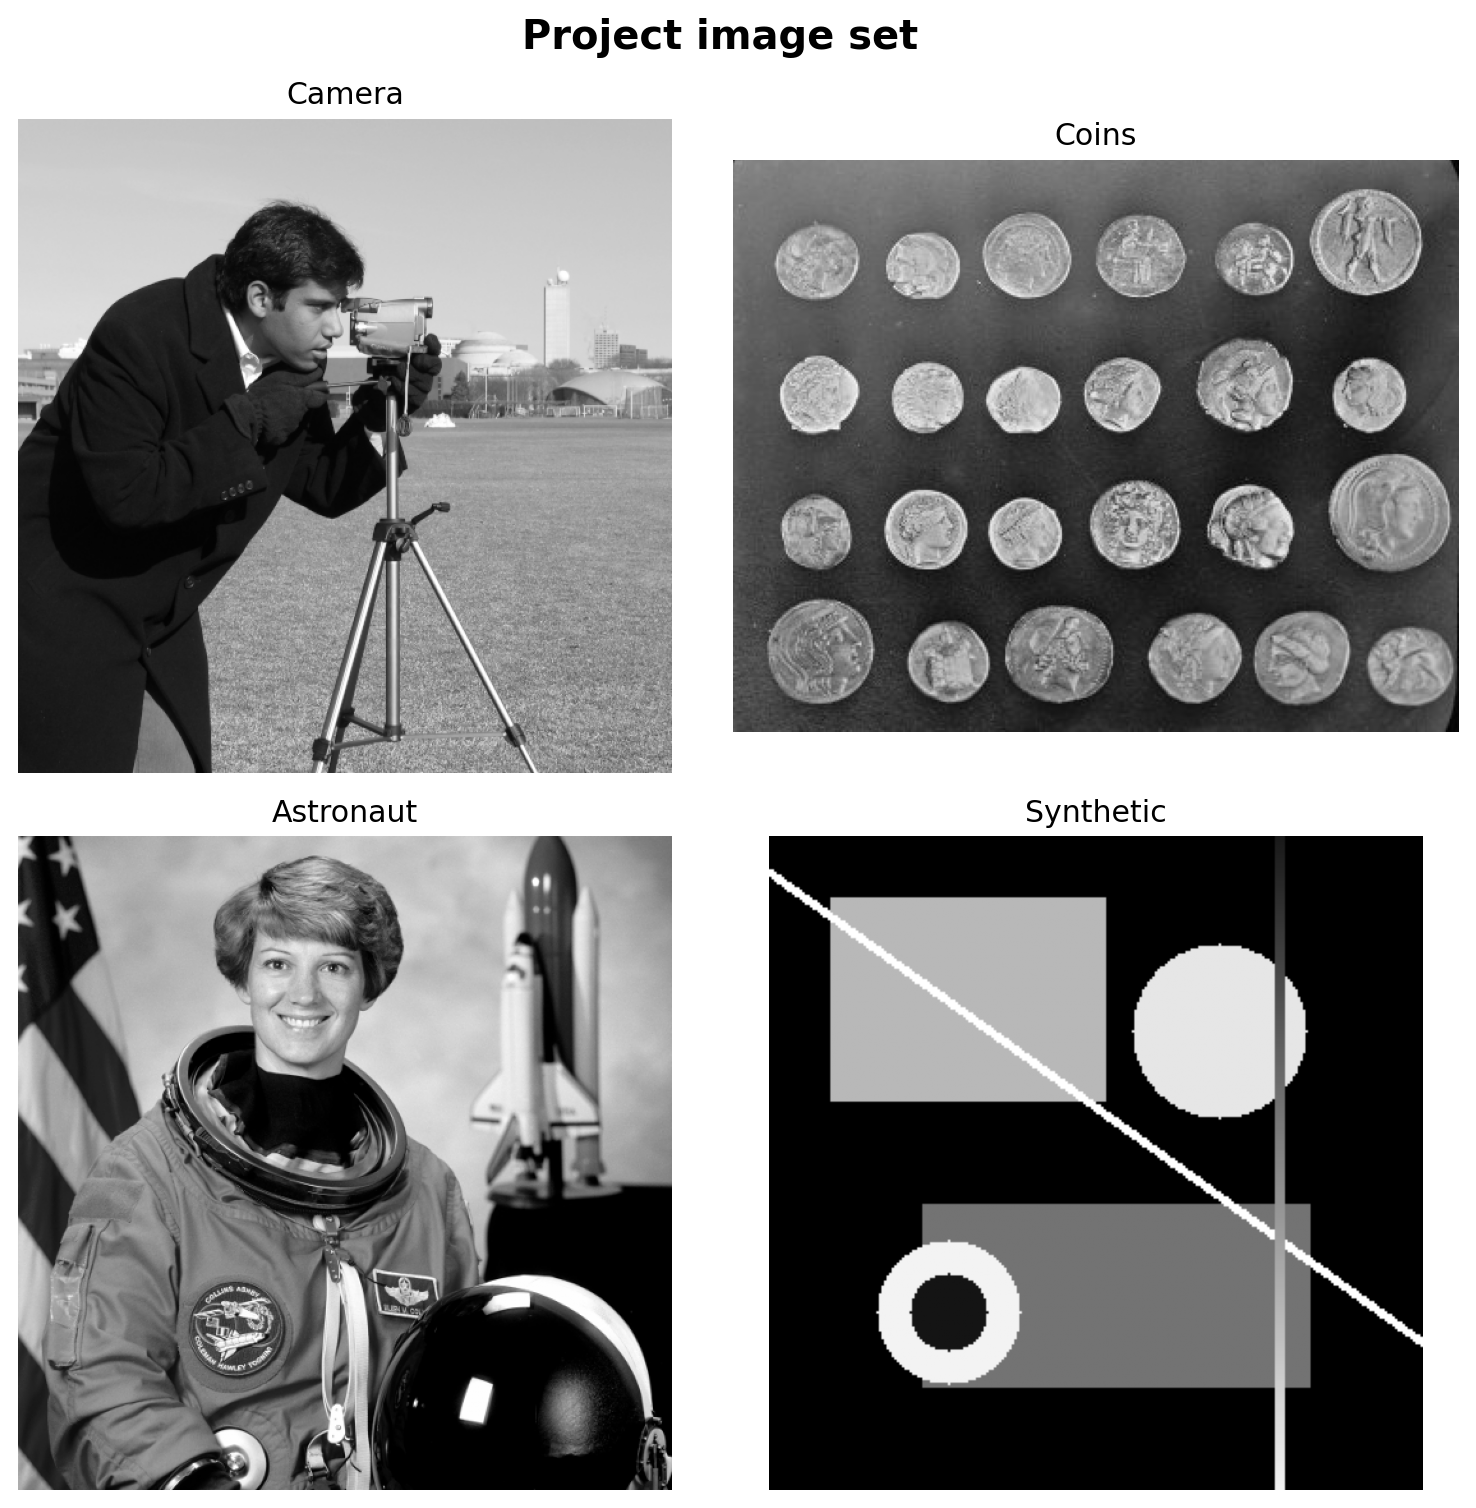
\includegraphics[width=0.42\linewidth,height=0.48\textheight,keepaspectratio]{../assets/generated/figures/image_gallery.png}
\end{frame}

\begin{frame}[t]{2D Convolution and Sobel Intuition}
  \justifying
  \small
  \begin{columns}[T]
    \column{0.55\linewidth}
    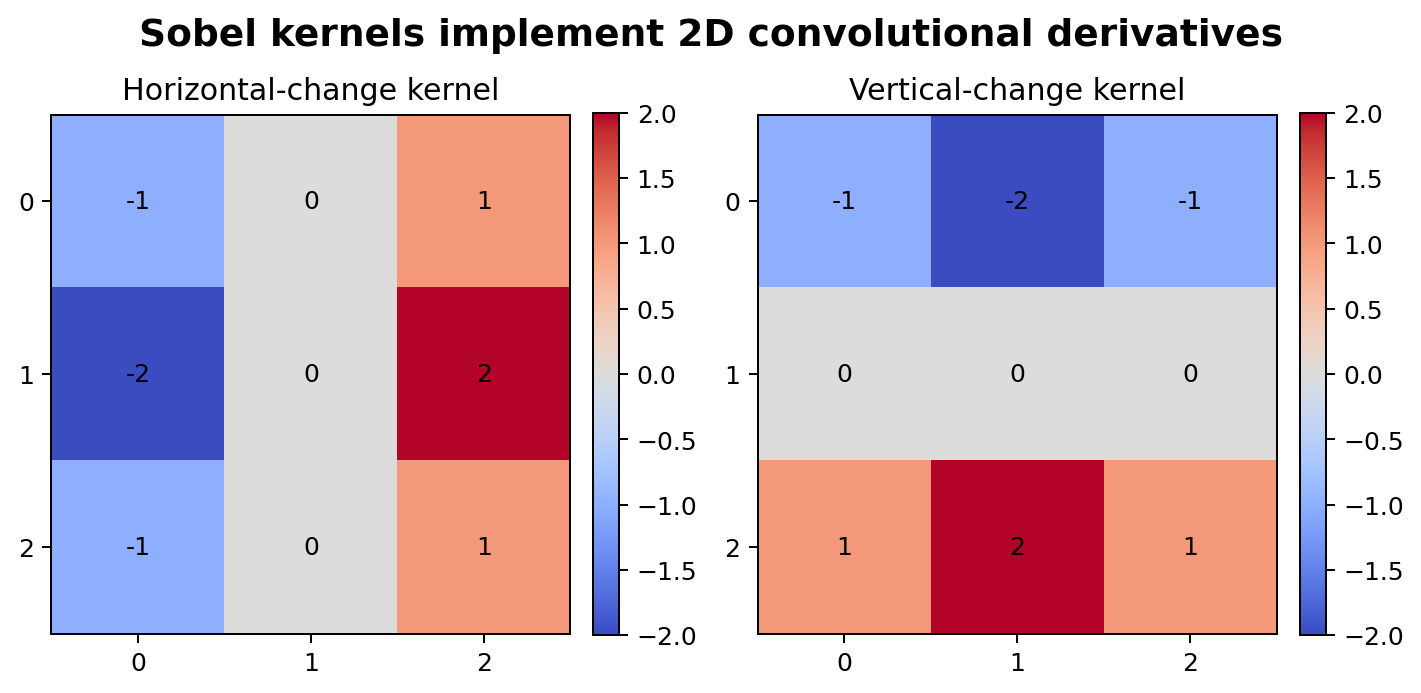
\includegraphics[width=\linewidth,height=0.54\textheight,keepaspectratio]{../assets/generated/figures/sobel_kernels.png}
    \column{0.42\linewidth}
    \begin{itemize}
      \item Sobel uses two convolution kernels.
      \item One estimates horizontal change.
      \item One estimates vertical change.
      \item The gradient magnitude highlights boundaries.
    \end{itemize}
  \end{columns}
\end{frame}

\begin{frame}[t]{Failure Case: Noise Corrupts Edges}
  \centering
  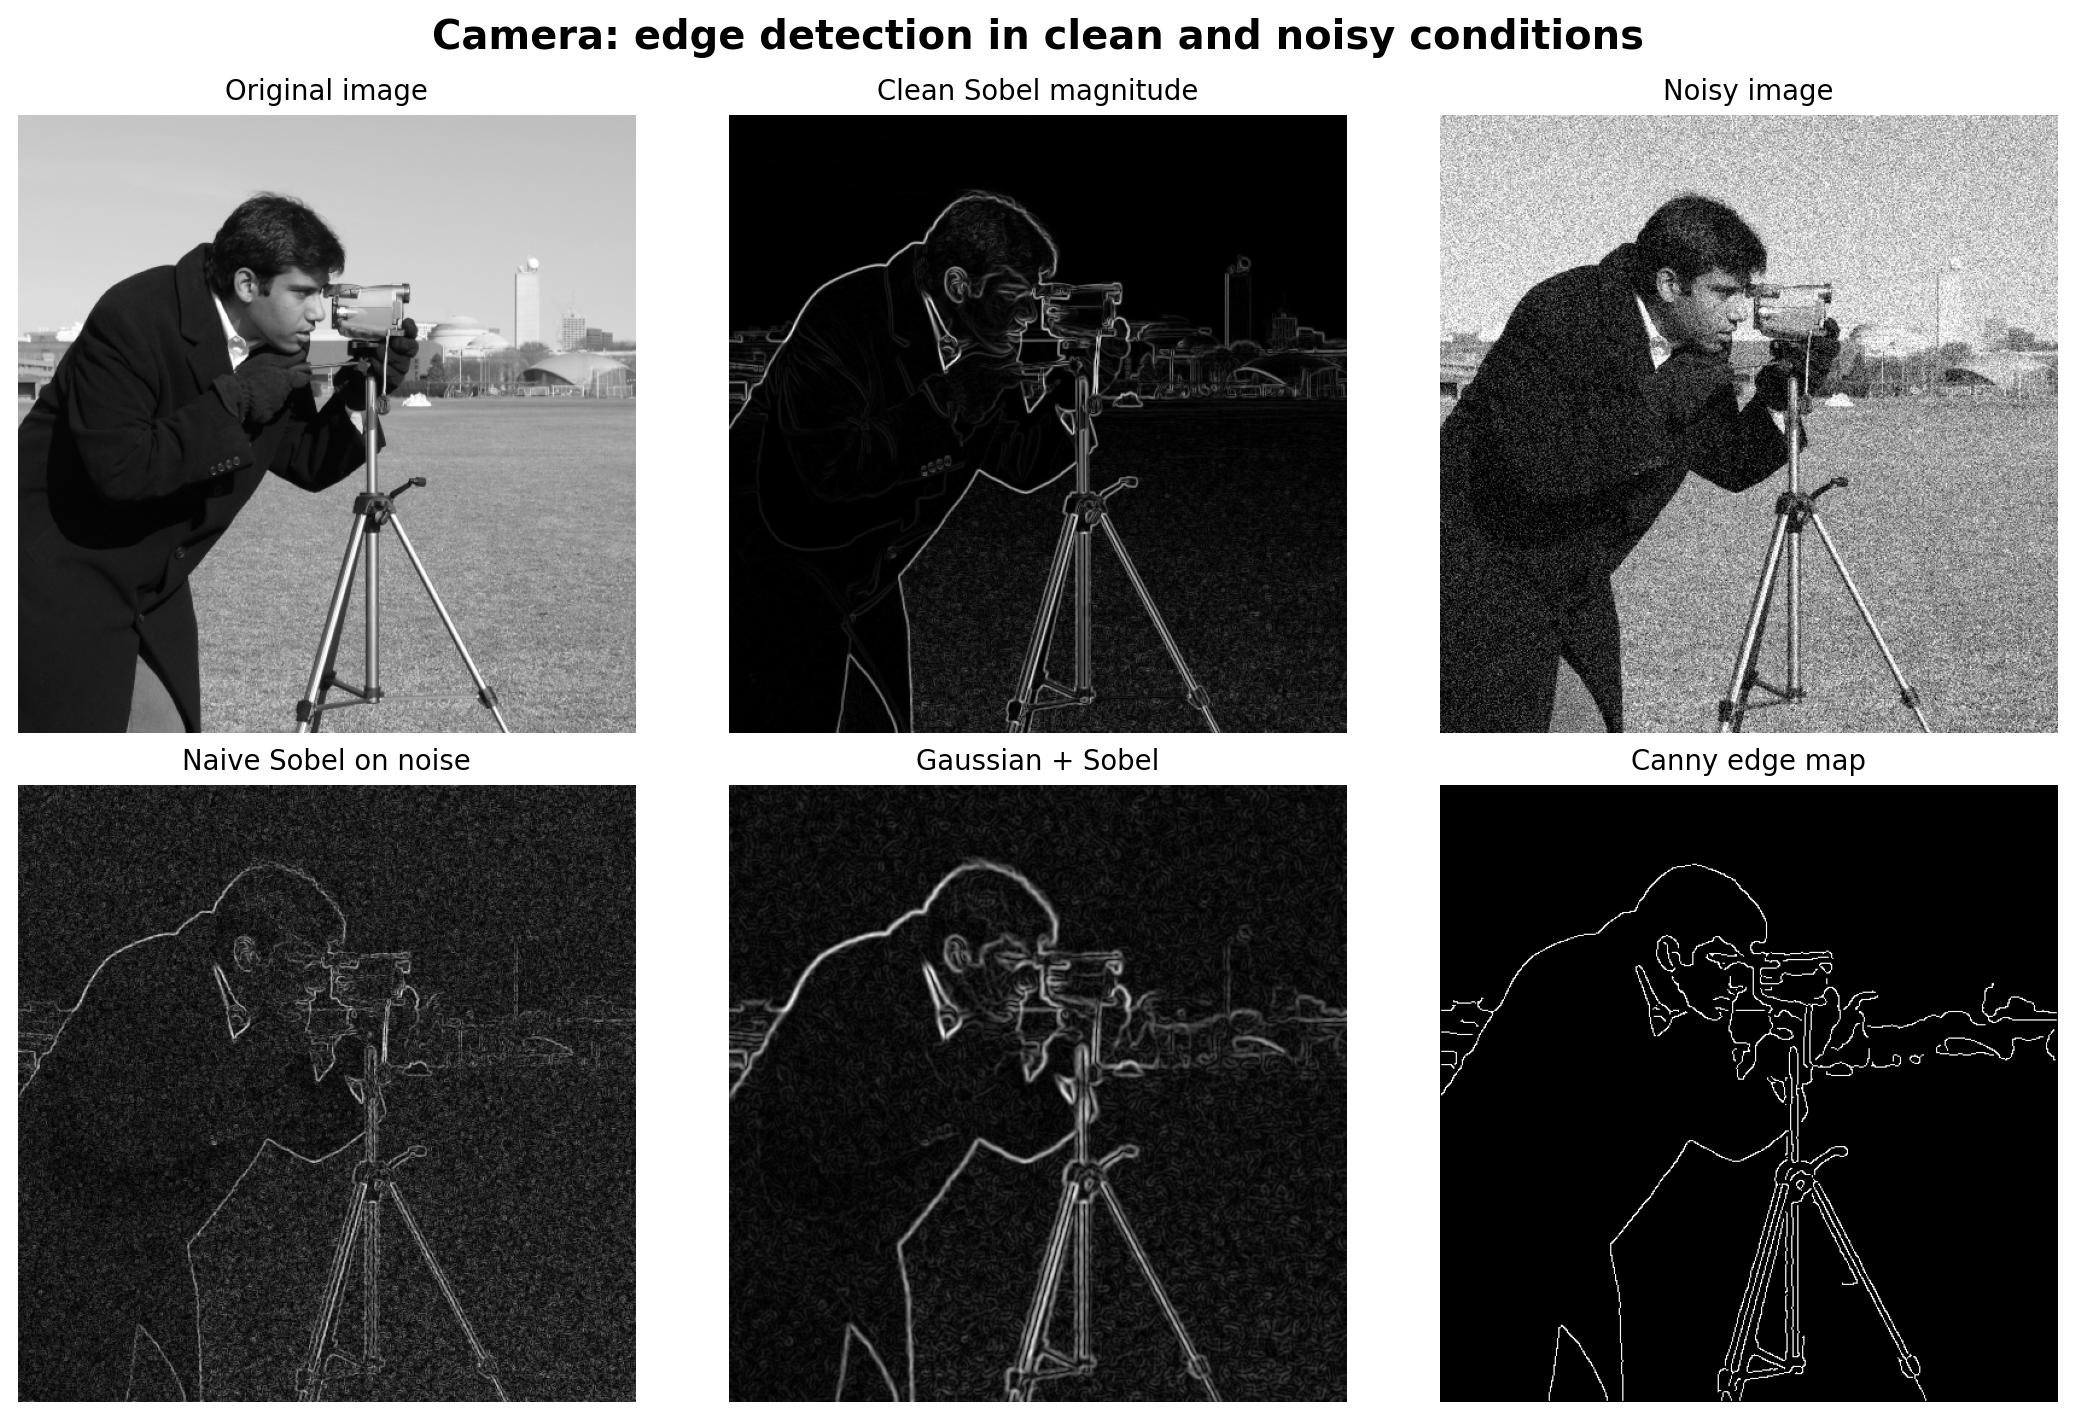
\includegraphics[width=0.94\linewidth,height=0.71\textheight,keepaspectratio]{../assets/generated/figures/camera_pipeline.png}
\end{frame}

\begin{frame}[t]{Fix: Smooth Before Differentiating}
  \justifying
  \small
  \begin{columns}[T]
    \column{0.44\linewidth}
    \begin{itemize}
      \item Gaussian smoothing suppresses unstable high-frequency noise.
      \item Sobel after smoothing recovers stronger large-scale boundaries.
      \item Too much smoothing also erases weak detail.
    \end{itemize}
    \column{0.53\linewidth}
    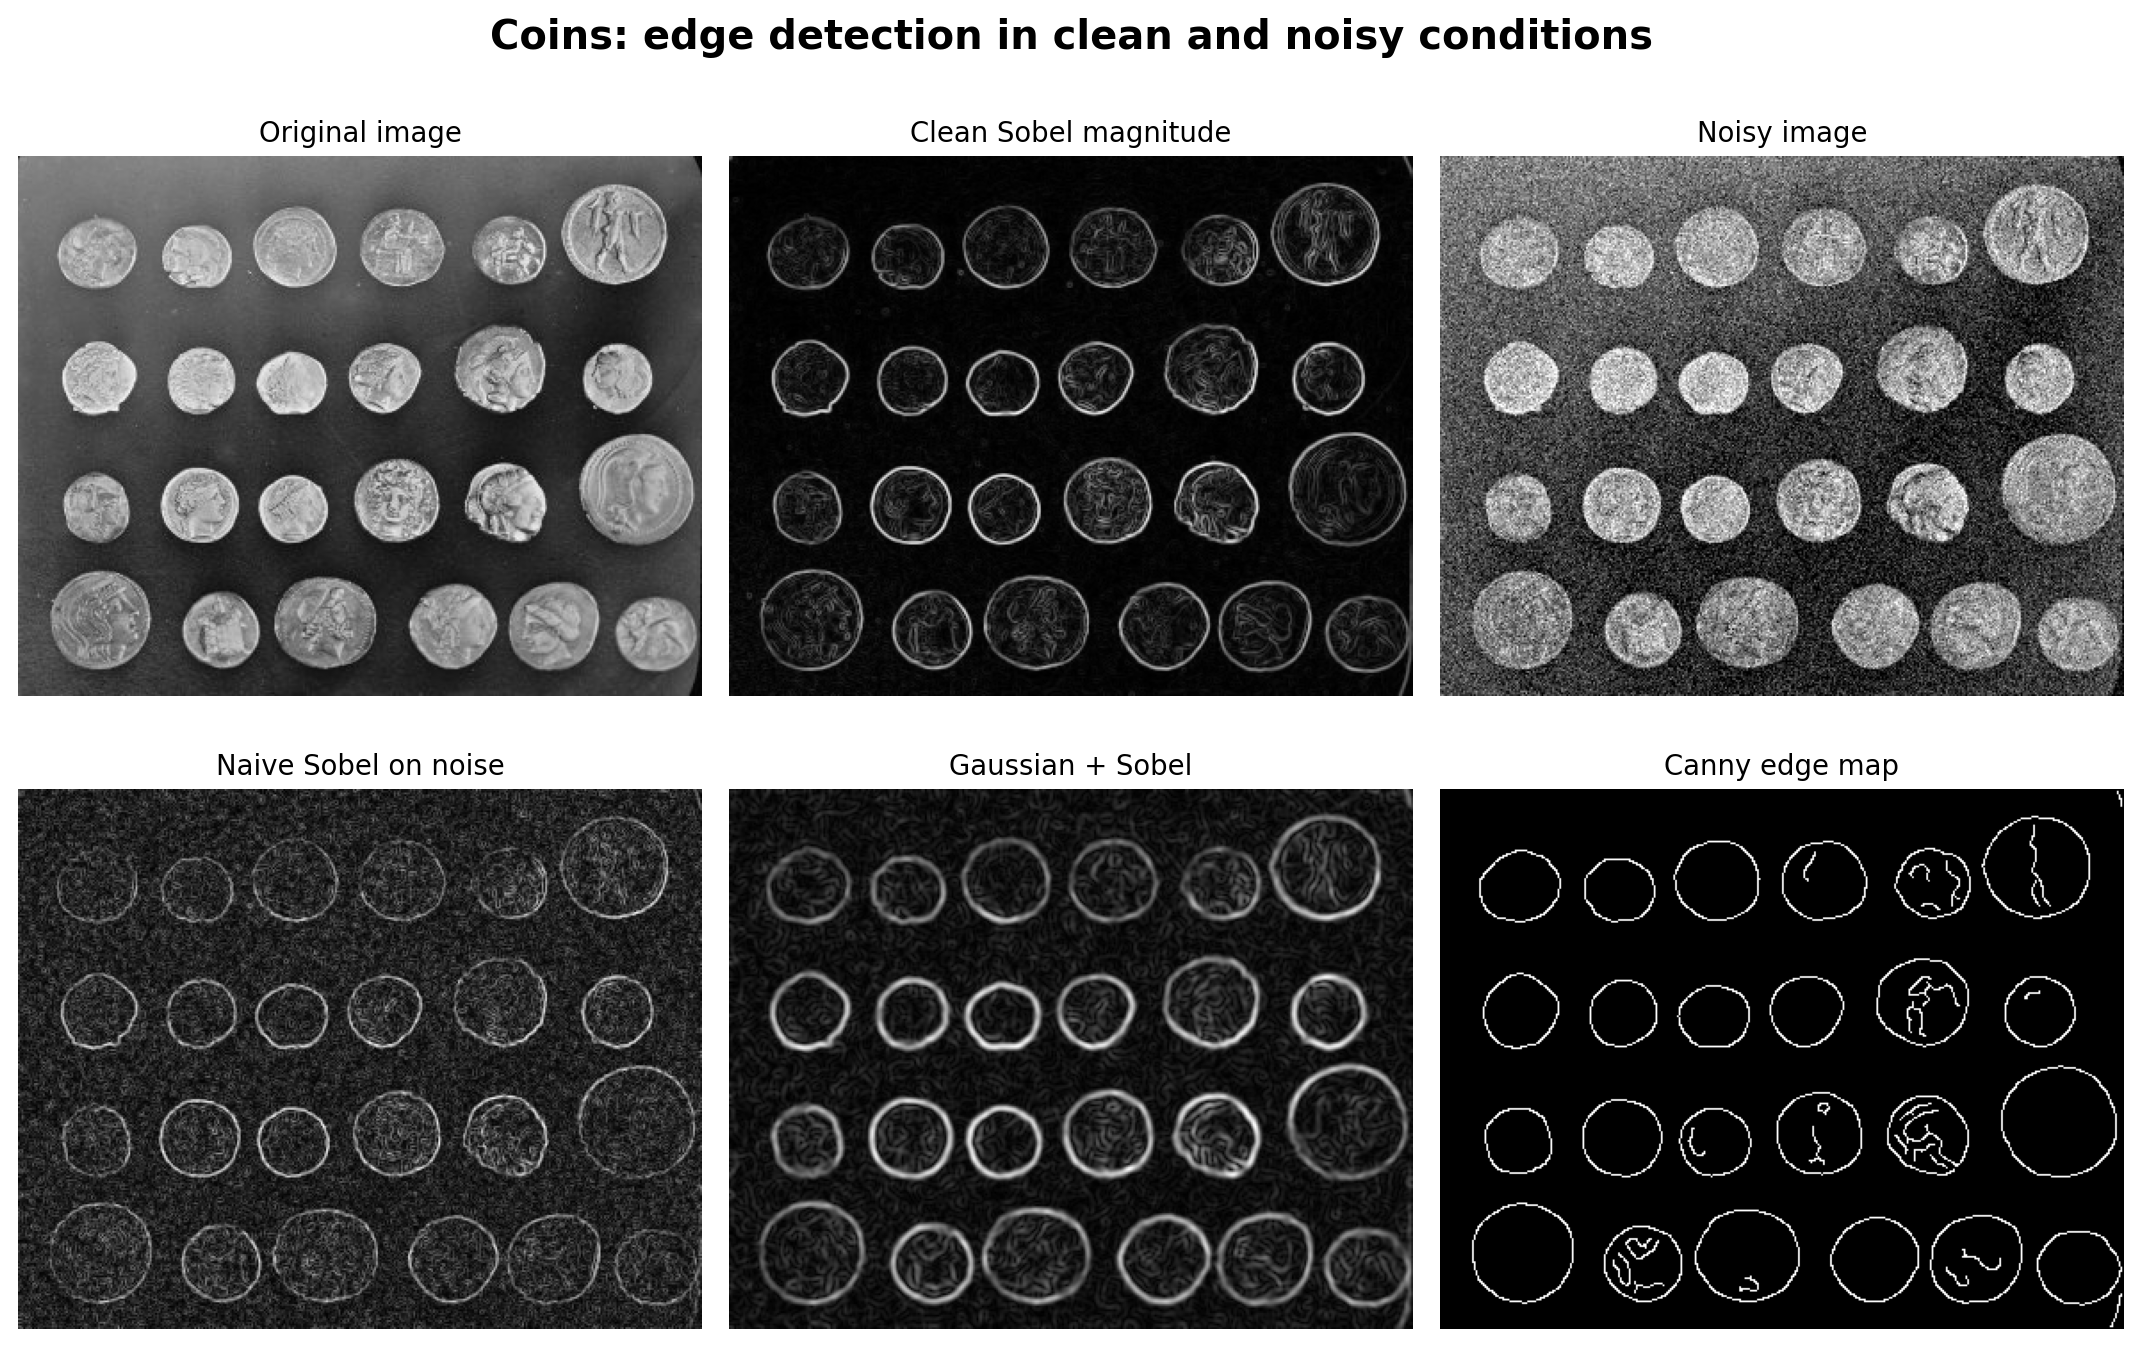
\includegraphics[width=\linewidth,height=0.58\textheight,keepaspectratio]{../assets/generated/figures/coins_pipeline.png}
  \end{columns}
\end{frame}

\begin{frame}[t]{Canny as a Refined Pipeline}
  \justifying
  \small
  \begin{columns}[T]
    \column{0.48\linewidth}
    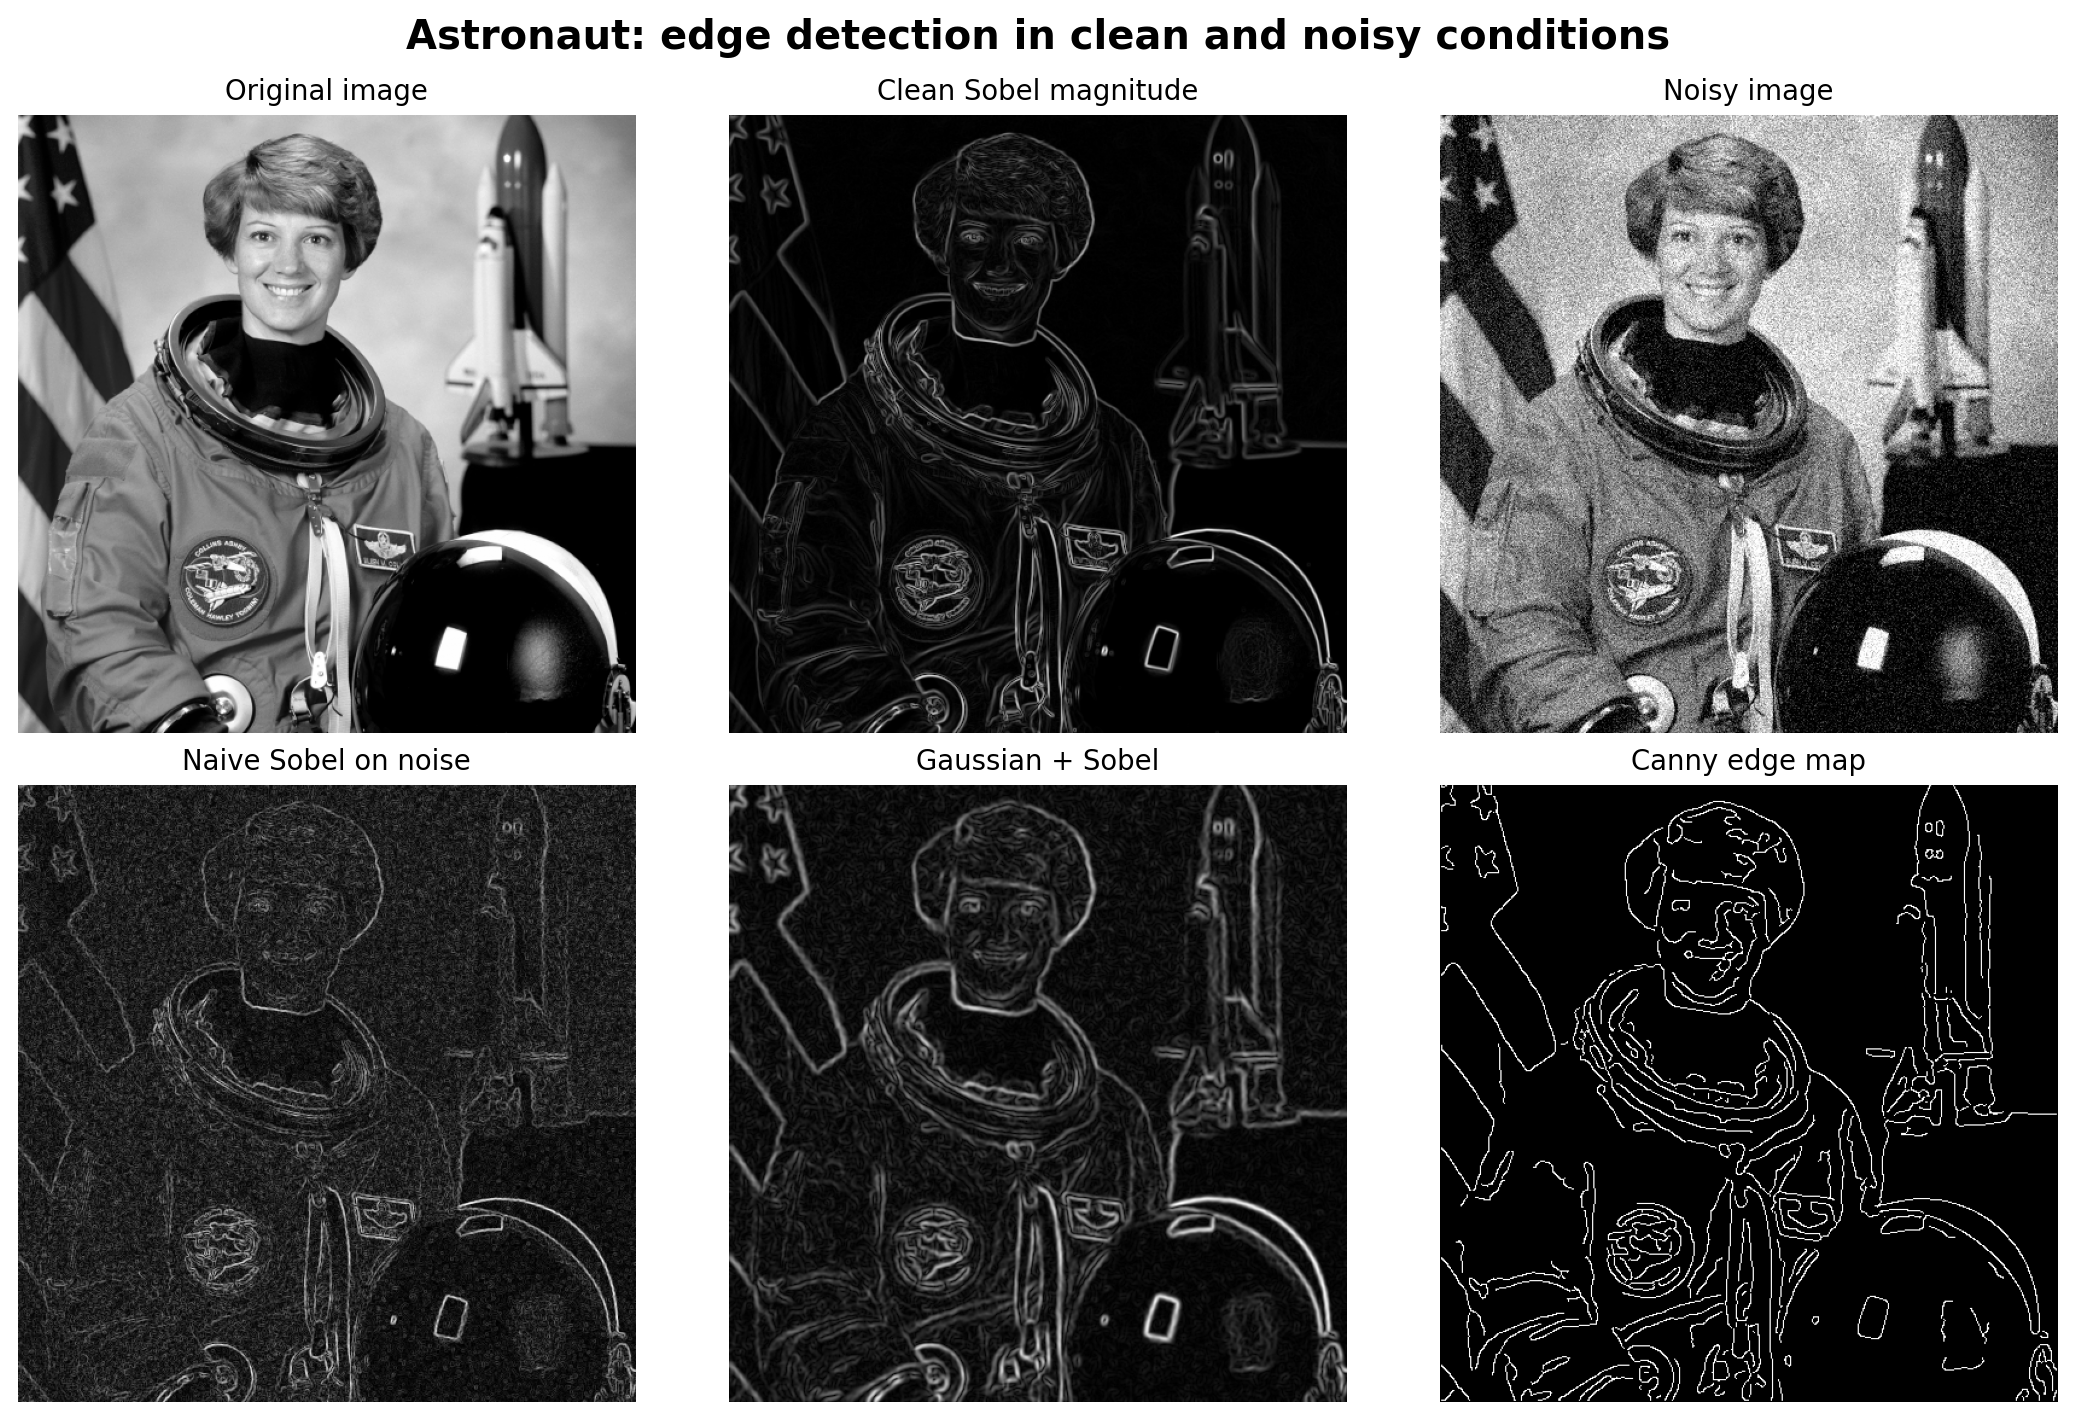
\includegraphics[width=\linewidth,height=0.58\textheight,keepaspectratio]{../assets/generated/figures/astronaut_pipeline.png}
    \column{0.46\linewidth}
    \begin{itemize}
      \item Canny combines smoothing, gradients, suppression, and thresholding.
      \item It is stronger than raw Sobel.
      \item But it still depends on the same filtering logic.
    \end{itemize}
  \end{columns}
\end{frame}

\begin{frame}[t]{Tradeoff Heatmap}
  \justifying
  \small
  \centering
  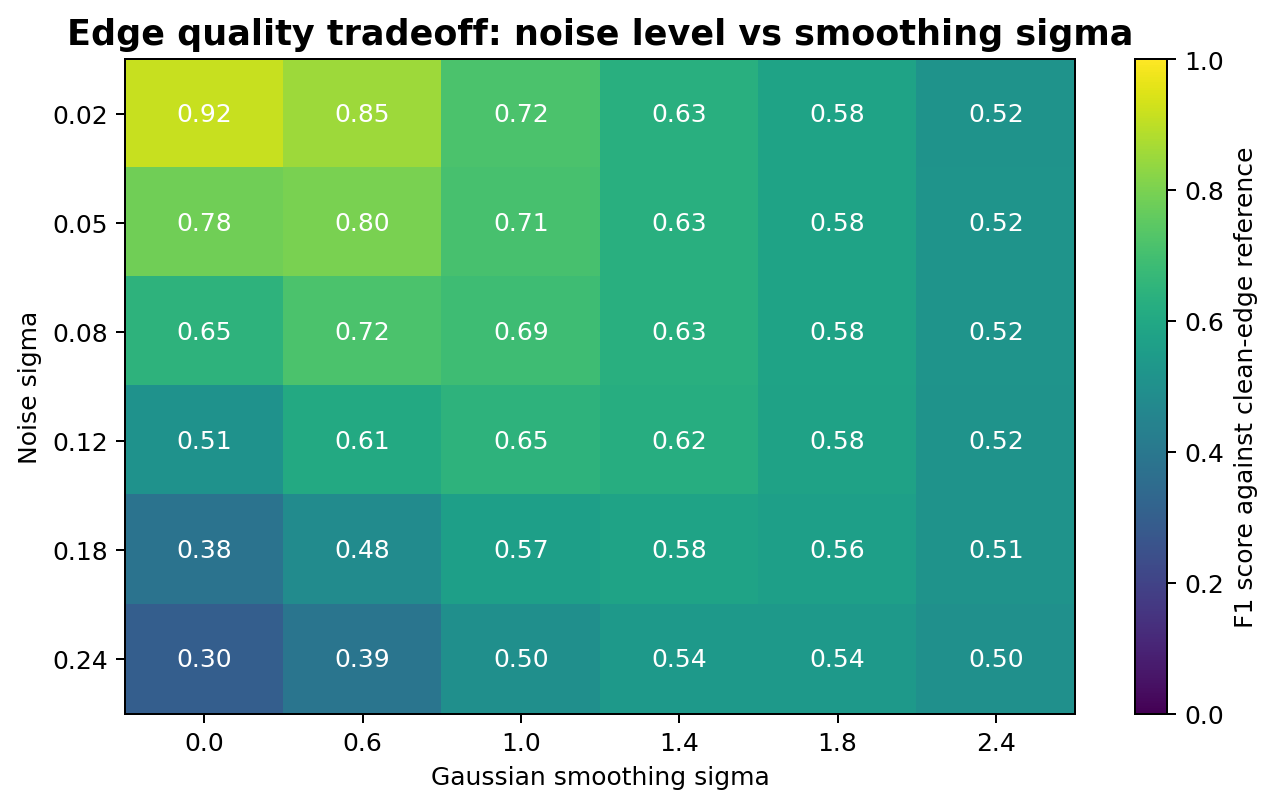
\includegraphics[width=0.74\linewidth,height=0.58\textheight,keepaspectratio]{../assets/generated/figures/tradeoff_heatmap.png}
  \vspace{0.2em}
  
  Higher noise usually needs more smoothing, but oversmoothing removes useful edges.
\end{frame}

\begin{frame}{CNN and Diffusion Connection}
  \justifying
  \begin{itemize}
    \item Early CNN filters often learn edge-like patterns.
    \item Diffusion models repeatedly remove noise from an image estimate.
    \item Neither idea replaces classical filtering intuition.
    \item They extend it.
  \end{itemize}
\end{frame}

\begin{frame}{Conclusion}
  \justifying
  \begin{itemize}
    \item Edge detection is a filtering problem, not a black box.
    \item Noise breaks naive derivatives because both noise and edges are high-frequency.
    \item Pre-smoothing improves robustness, but detail is the cost.
    \item The same logic carries forward into modern vision systems.
  \end{itemize}
\end{frame}

\begin{frame}[t]{References}
  \footnotesize
  \begin{enumerate}
    \item ECE 0402 course project guideline.
    \item scikit-image: Canny edge detector.
    \item scikit-image API: filters.
    \item HIPR2: Sobel Edge Detector.
    \item HIPR2: Canny Edge Detector.
    \item B. P. Lathi, \textit{Linear Systems and Signals}.
    \item Luis F. Chaparro, \textit{Signals and Systems Using MATLAB}.
  \end{enumerate}
\end{frame}

\begin{frame}[t]{Team Responsibilities}
  \small
  \begin{tabular}{p{0.17\linewidth} p{0.29\linewidth} p{0.38\linewidth}}
    \toprule
    Member & Responsibility & Concrete Output \\
    \midrule
    Member A & Framing and references & Topic definition, slide story \\
    Member B & Implementation & Python modules, figures \\
    Member C & Validation & Heatmap analysis, checks \\
    Member D & Delivery & Slide edits, narration, rehearsal \\
    \bottomrule
  \end{tabular}
\end{frame}

\end{document}
